\section{File structure}
	\subsection{JSON file structure}
JSON files which contain trained algorithm definition must be structured as it follow.	

		\subsubsection{Linear Regression}
		\begin{itemize}
			\item\textbf{author}: the file's author. Set in defaul as "TeamAFK";
			\item\textbf{version}: the training tool application version. Set in deafult as "1.0.0";
			\item\textbf{algorithm}: the trained algorithm . Set in default as "Linear Regression"; 	
			\item\textbf{date}: the current date when file is created;
			\item\textbf{predictors}: list of all predictors' labels which are taken from CSV files;
			\item\textbf{result}: list of obtained coefficients from the training. In detail:
			\begin{itemize}
					\item\textbf{a}: list of coefficients values of the regression line formula;
					\item\textbf{b}: bias of the regression line formula;
				\end{itemize}
			\item\textbf{line}: regression line formula;
					
		\end{itemize}
		
		\begin{figure}[H]
		\centering
		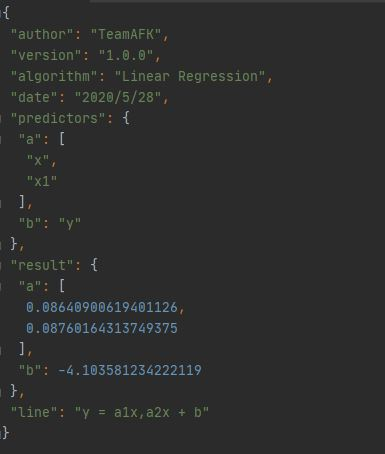
\includegraphics[scale=0.70]{../Developer_manual/img/linear_regression_json.JPG}
		\caption{Example of Linear Regression JSON file}
	\end{figure}	
	
		\subsubsection{Support Vector Machine}
		\begin{itemize}
			\item\textbf{author}: the file's author. Set in defaul as "TeamAFK";
			\item\textbf{version}: the training tool application version. Set in deafult as "1.0.0";
			\item\textbf{algorithm}: the trained algorithm . Set in default as "SVM"; 	
			\item\textbf{date}: the current date when file is created;
			\item\textbf{predictors}: list of all predictors' labels which are taken from CSV files;
			\item\textbf{result}: list of obtained coefficients from the training. In detail:
				\begin{itemize}
					\item\textbf{a}: list of weights values of the regression line formula;
					\item\textbf{b}: bias of the regression line formula;
				\end{itemize}
			\item\textbf{line}: separation line formula.
					
		\end{itemize}
		
		\begin{figure}[H]
		\centering
		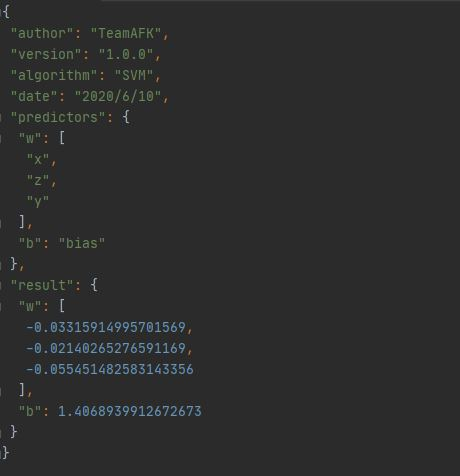
\includegraphics[scale=0.70]{../Developer_manual/img/support_vector_machine_json.JPG}
		\caption{Example of Linear Regression JSON file}
	\end{figure}	
		
	
	\subsection{CSV file structure}
Weather you use choose to train one algorithm intead of another one CSV file has a common structure:
	\begin{itemize}
		\item\textbf{first columns till y column}: each column represents a predictor;
		\item\textbf{y}: this column contains the results.	
	\end{itemize}	 

First line of CSV files must contain predictors tags while the other lines contain values. If you want to add a predictor you must insert a column, before y column, with the predictor tag as first line.

\begin{figure}[H]
		\centering
		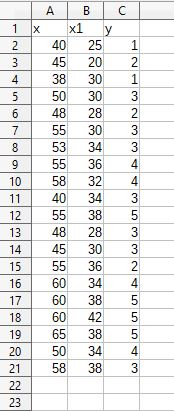
\includegraphics[scale=0.70]{../Developer_manual/img/linear_regression_csv.JPG}
		\caption{Example of Linear Regression CSV file}
	\end{figure}

In SVM CSV files you can find one more column named "label" which contains the data group. 

\begin{figure}[H]
		\centering
		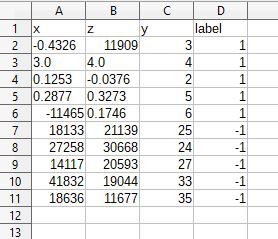
\includegraphics[scale=0.70]{../Developer_manual/img/support_vector_machine_csv.JPG}
		\caption{Example of Linear Regression CSV file}
	\end{figure}
 



